%
% teil1.tex -- Beispiel-File für das Paper
%
% (c) 2020 Prof Dr Andreas Müller, Hochschule Rapperswil
%
% !TEX root = ../../buch.tex
% !TEX encoding = UTF-8
%
\section{Allgemeiner Aufbau einer Möbius Transformation
\label{moebius:section:teil1}}
\kopfrechts{Allgemeiner Aufbau einer Möbius Transformation}

Eine Möbius Transformation kann man als Kombinationen von einfachen Transformationen verstehen.
Es gibt drei Arten von diesen Transformationen.
\index{Mobius-Transformation@Möbius-Transformation}%

\subsubsection{Die Translation}
Eine Translation wird durch die Abbildung
\[
z \mapsto z + b
\]
beschrieben.
Sie verschiebt jeden Punkt der komplexen Ebene um die komplexe Zahl b.

\begin{figure}
	\centering
	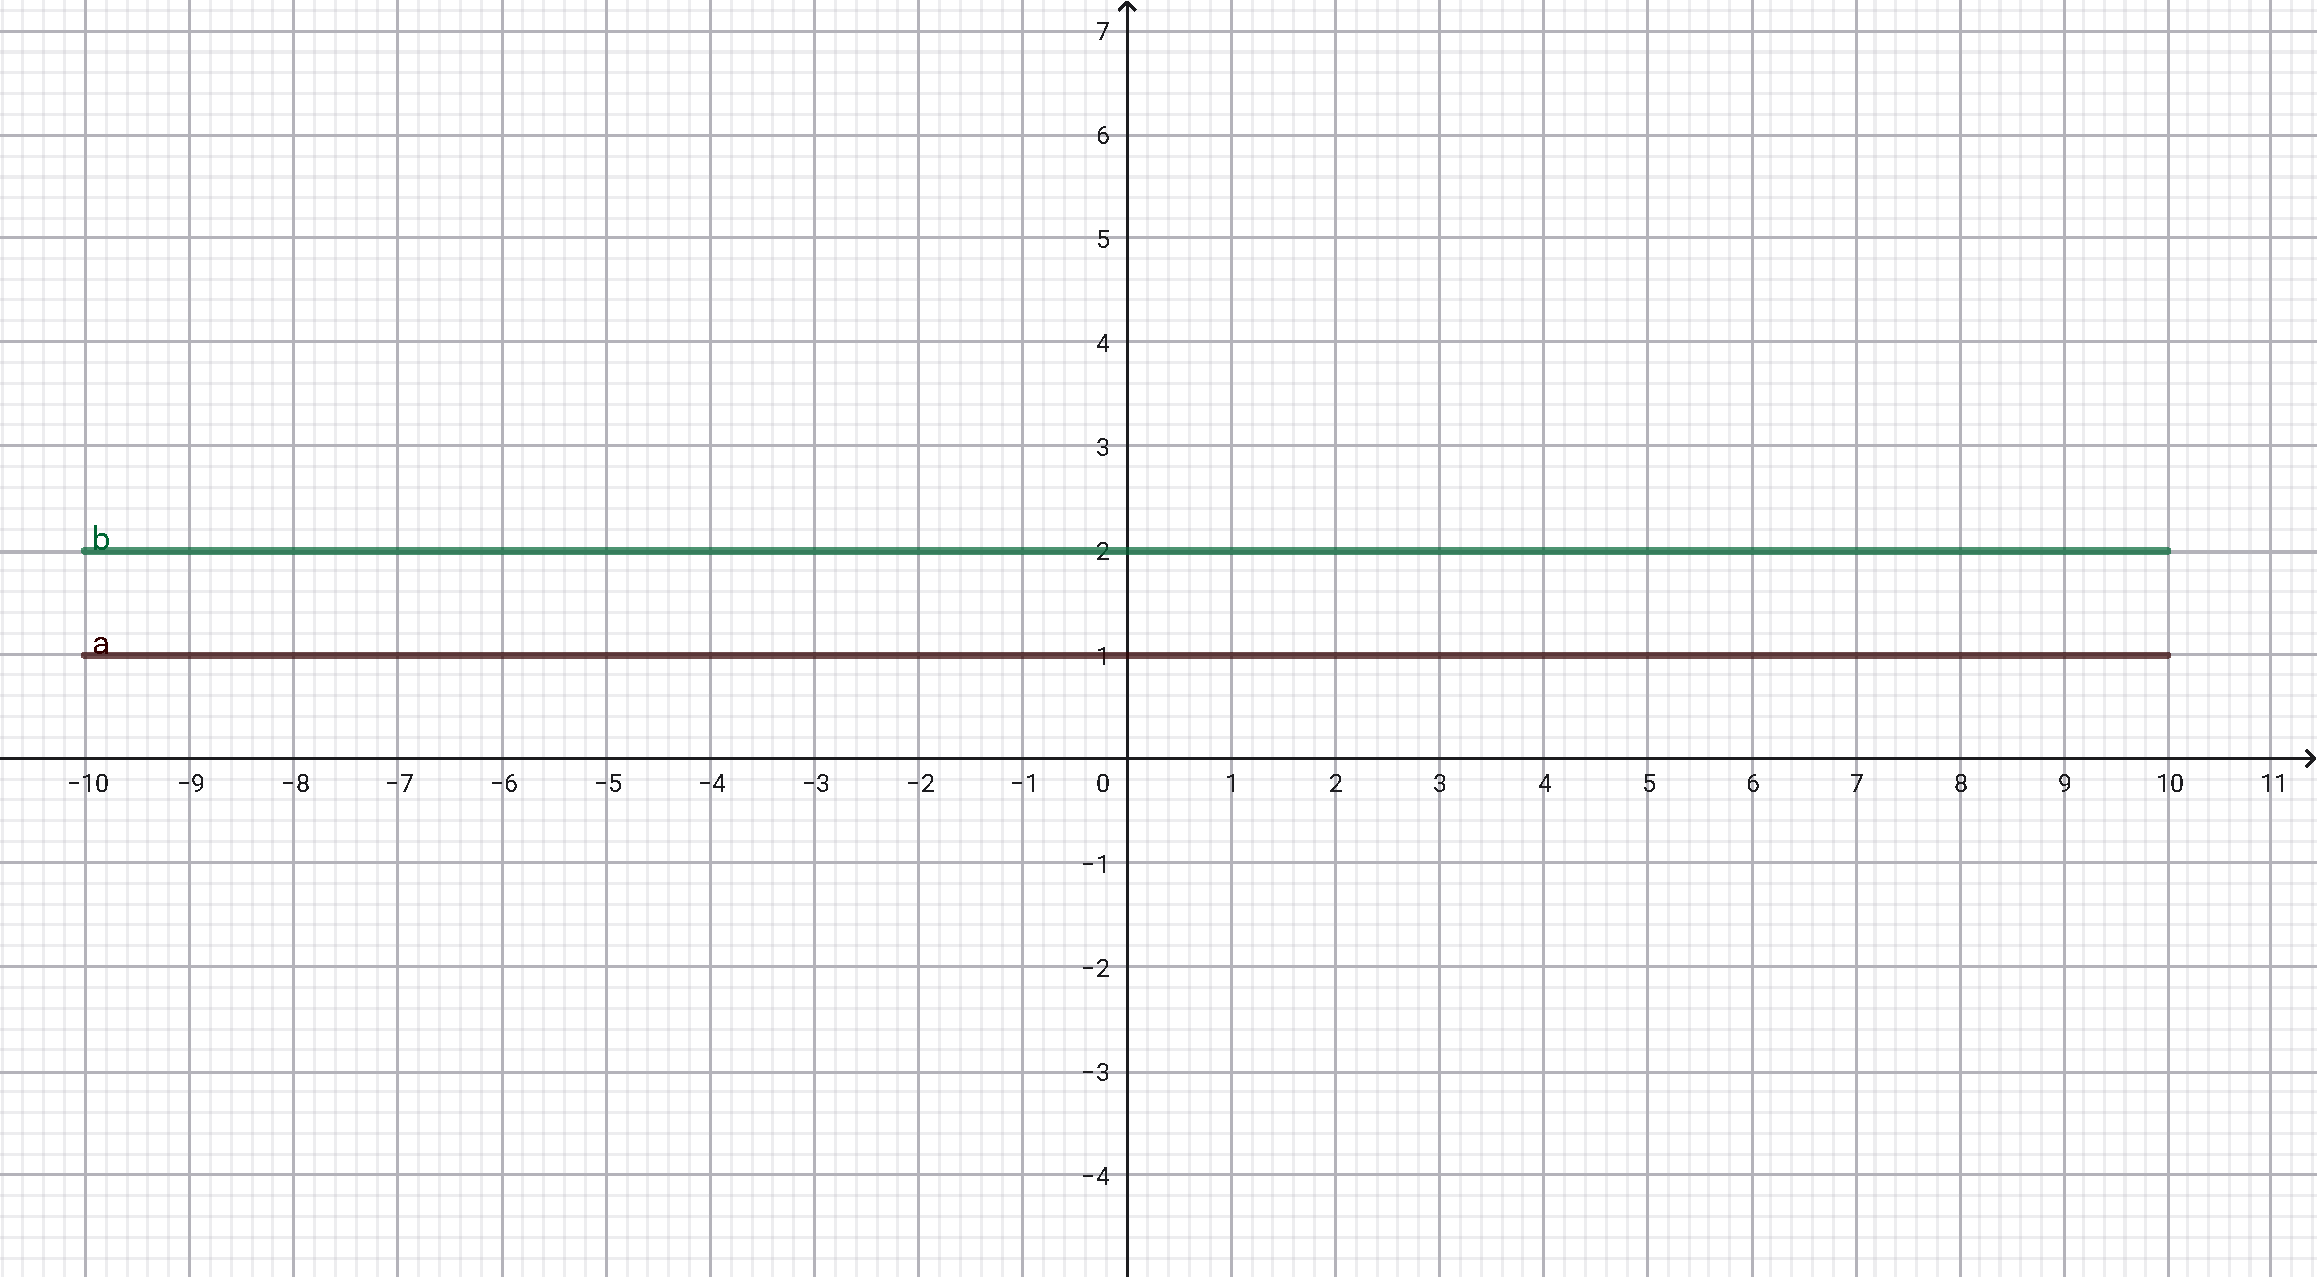
\includegraphics[width=1\textwidth]{papers/moebius/bild5.pdf}
	\caption{Verschiebung des Imaginärteils (erstellt mit GeoGebra)}
\end{figure}
\index{GeoGebra}%


\subsubsection{Drehstreckung}
Die Drehstreckung wird durch die Abbildung
\[
z \mapsto az
\]
beschrieben.
Diese Transformation beschreibt eine Streckung und gleichzeitig eine Rotation der komplexen Ebene um den Ursprung.
\index{Rotation}%
\begin{figure}
	\centering
	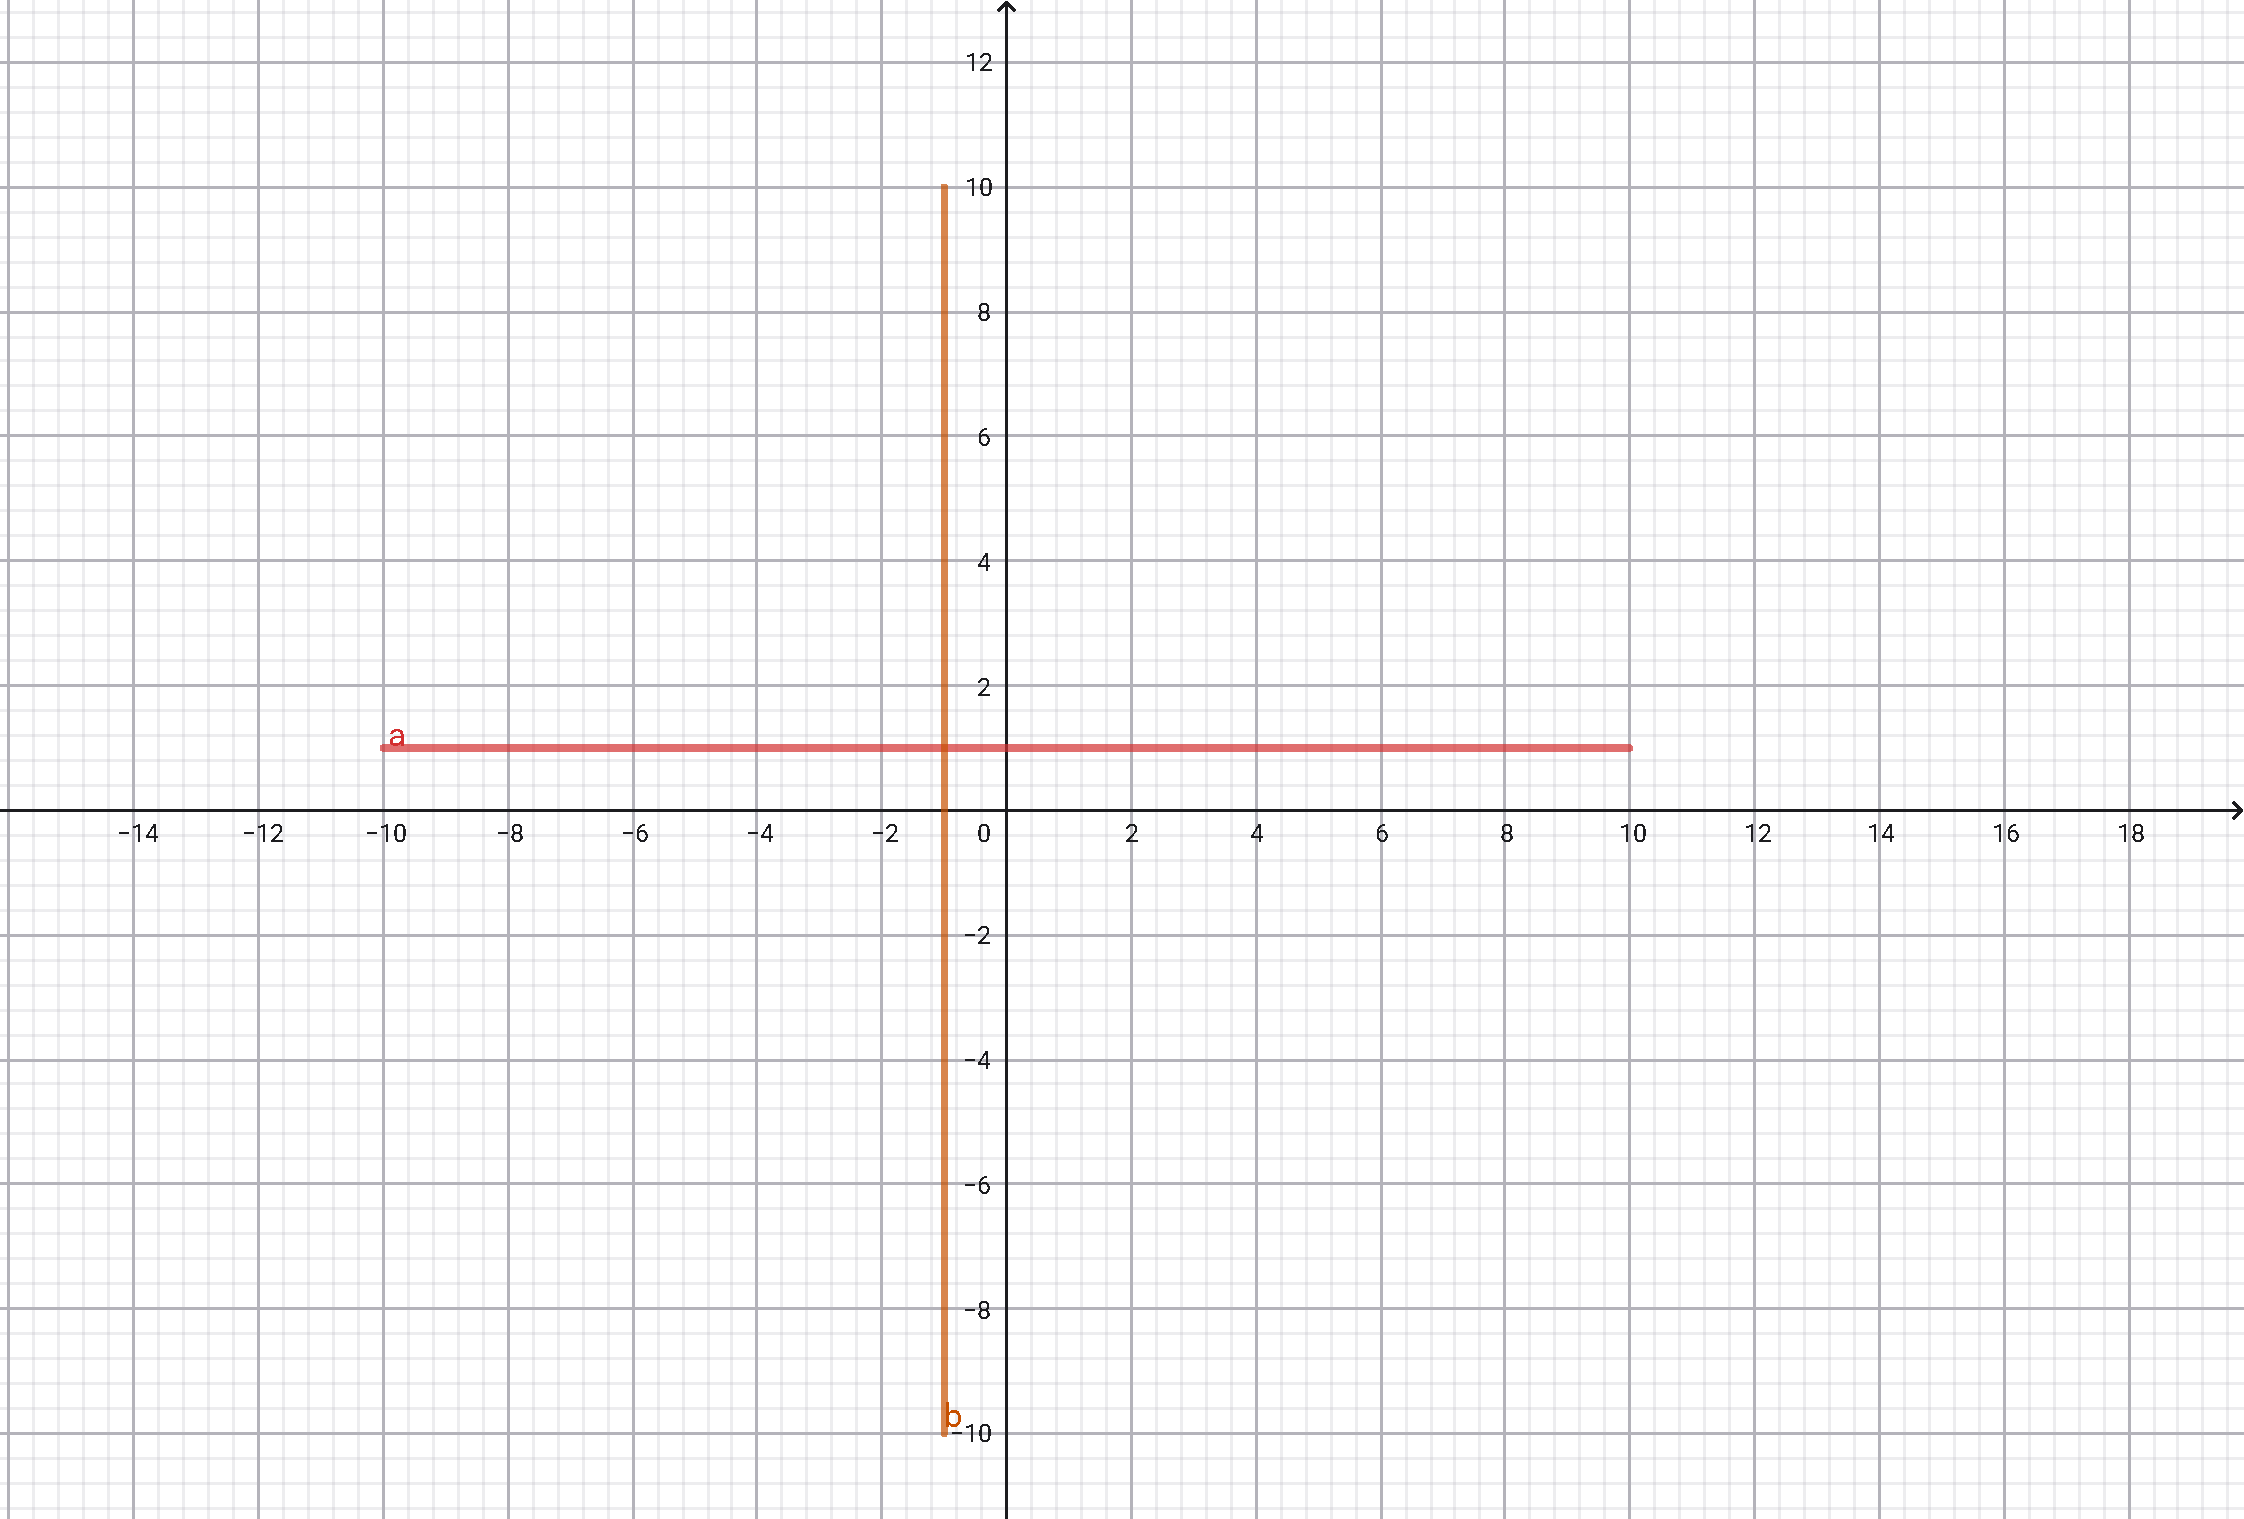
\includegraphics[width=1\textwidth]{papers/moebius/bild3.pdf}
	\caption{Drehung um 90 Grad (erstellt mit GeoGebra)}
\end{figure}
Für die Rotation wird für $a = e^{i\varphi}$ eingesetzt.

\subsubsection{Die Inversion}
Die Inversion wird durch die Abbildung
\index{Inversion}%
\[
z \mapsto \frac{1}{z}
\]
beschrieben.
Sie bildet jeden Punkt der komplexen Ebene auf seinen Kehrwert ab und ist verantwortlich für die charakteristische Abbildung von Geraden auf Kreise und umgekehrt.

\begin{figure}
	\centering
	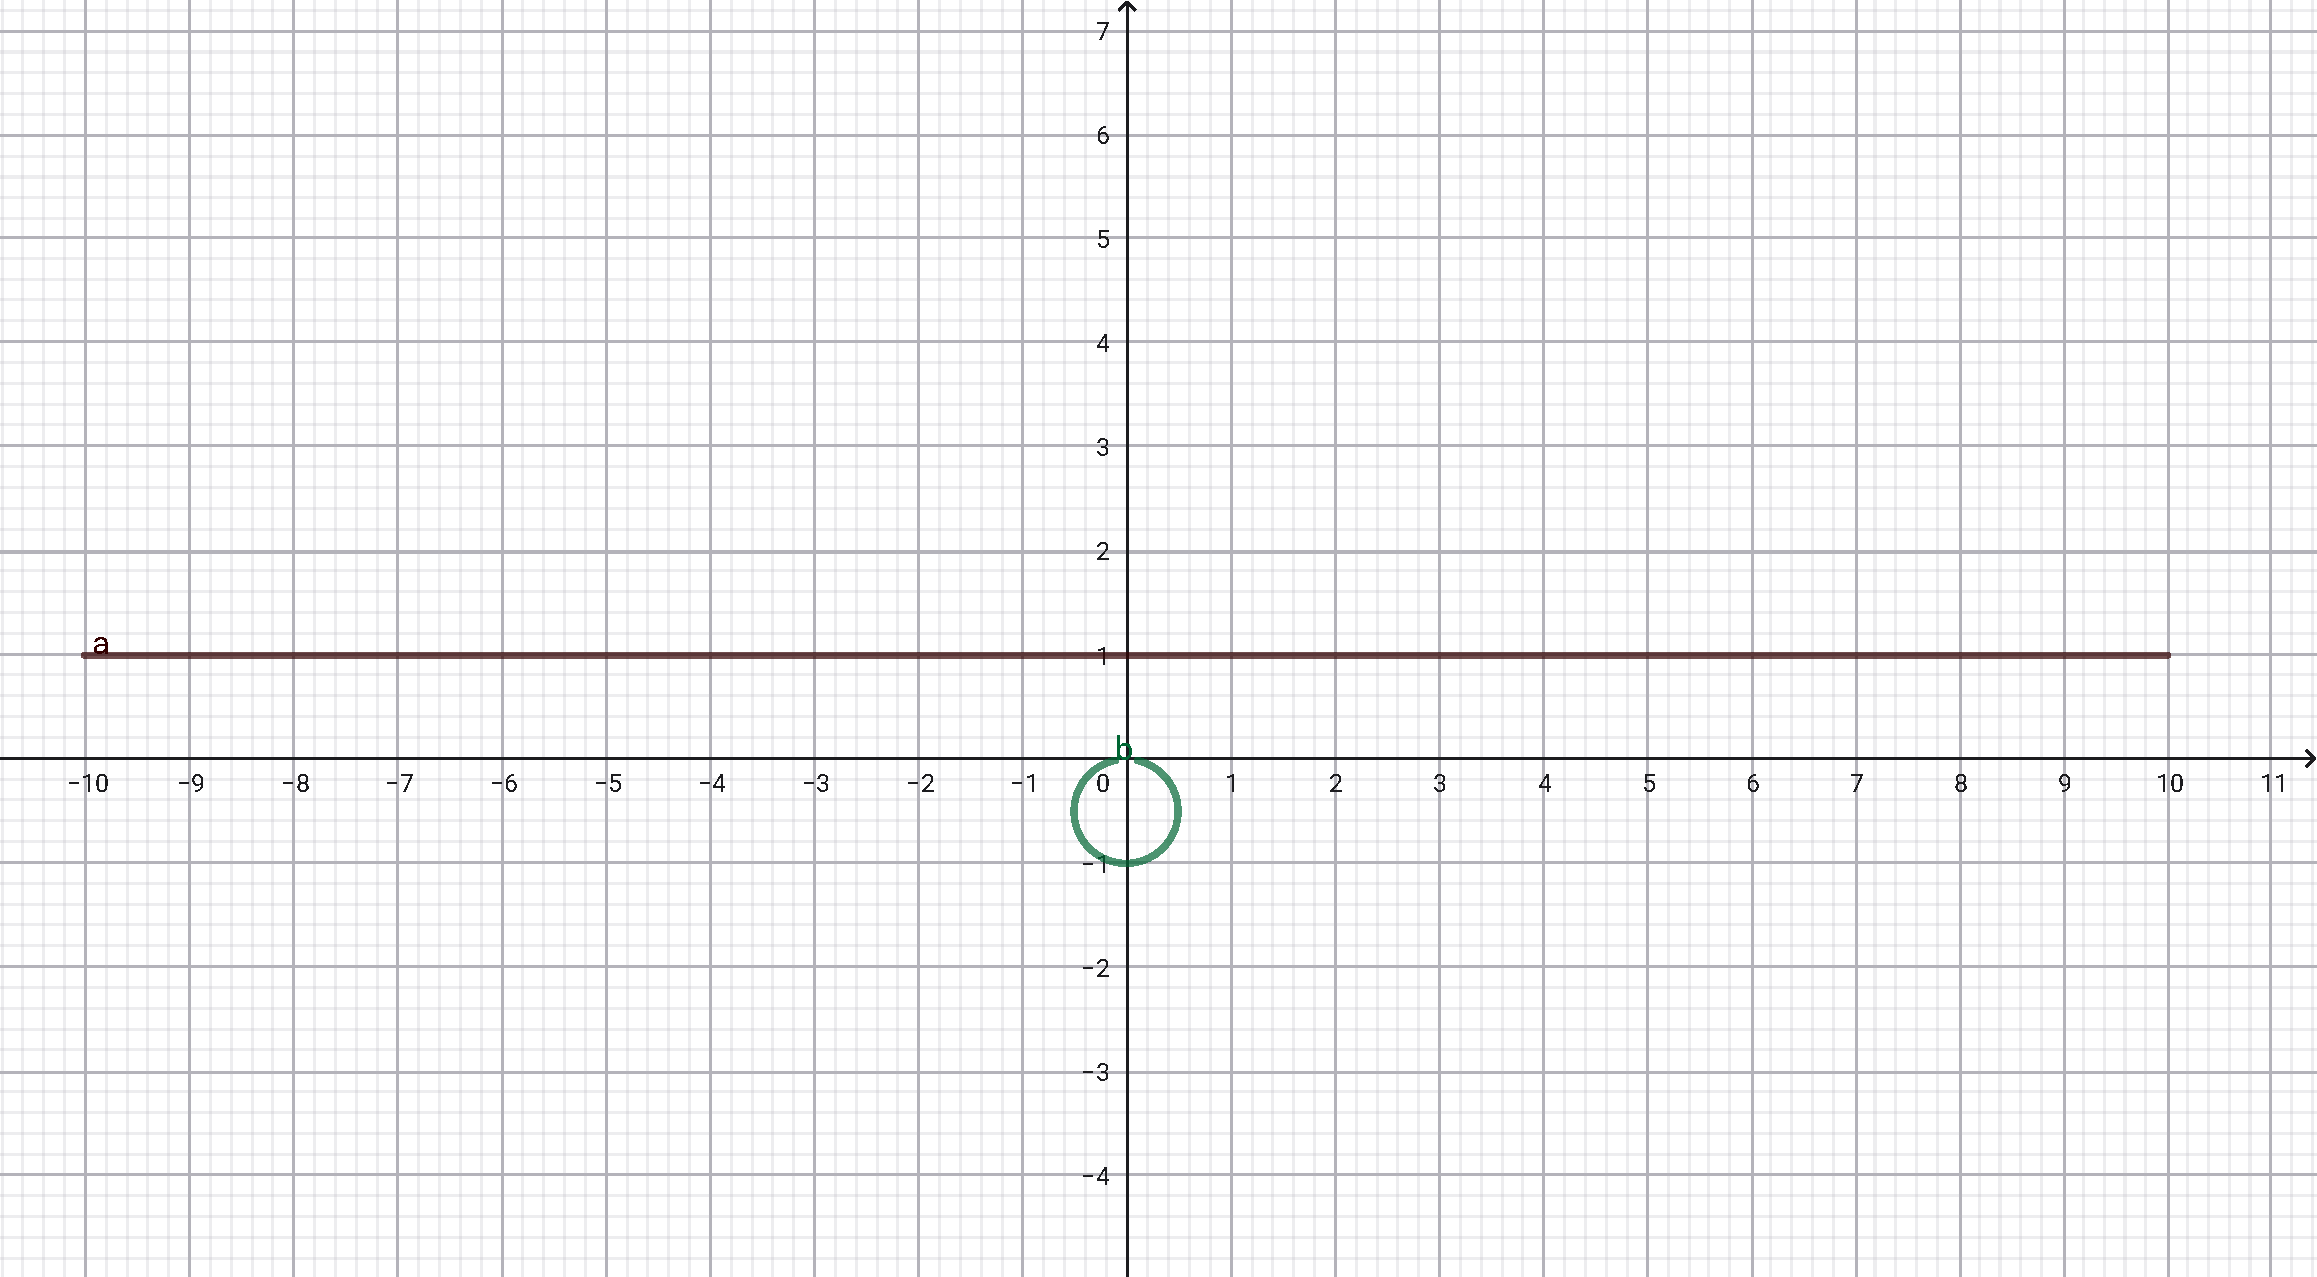
\includegraphics[width=1\textwidth]{papers/moebius/bild4.pdf}
	\caption{Gerade zu Kreis (erstellt mit GeoGebra)}
\end{figure}


\subsubsection{Die allgemeine Form einer Möbius-Transformation}

\[
f(z) = \frac{a z + b}{c z + d}, \quad a,b,c,d \in \mathbb{C}, \; ad - bc \neq 0
\]
kann als Verkettung von Translation, Drehstreckung und Inversion verstanden werden \cite{moebius:Moebiustransformationen}.
\[ad - bc \neq 0\]
Dies ist notwendig, da die Transformation sonst degeneriert. Für \(ad - bc = 0\) wäre die Abbildung nicht mehr invertierbar und würde die gesamte Ebene auf eine konstante oder eindimensionale Menge abbilden.
Möbius-Transformationen sind bijektiv.
Das bedeutet, dass sie sowohl injektiv als auch surjektiv sind:
\begin{itemize}
	\item Eine Funktion ist \emph{injektiv}, wenn verschiedene Punkte der Definitionsmenge auf verschiedene Punkte abgebildet werden.
\index{injektiv}%
	\item Eine Funktion ist \emph{surjektiv}, wenn jeder Punkt der Zielmenge von mindestens einem Punkt der Definitionsmenge getroffen wird.
\index{surjektiv}%
\end{itemize}
Damit ist jede Möbius-Transformation umkehrbar, d.\,h.~es existiert eine inverse Möbius-Transformation.
